\chapter{Instance Creation}
\label{ch:instance_creation}

In the following we explain, how the test instances are created. This concerns the sets of customers, routes, trips, vehicles and refuel points. Also the computation of the distances, times, costs and fuel states is discussed here. 

\section{Available Data}

As the mathematical content of this thesis is based on two previous theses \cite{Kaiser} and \cite{Knoll}, we also use their data in order to test our solution approaches. There are two reasons that we cannot apply these test data directly. Firstly, the respective data fulfill the restrictions of the simplified problem setting. We need customers and routes that consist of more than one car trip in order to test all the abilities of the developed solution methods. Secondly, only exemplary instances that are strongly restricted in time are provided to us. Therefore we need to extract these exemplary instances in order to receive a full test instance. 

The available test data are historical data that have been provided by the car sharing supplier Car2Go. The refuel point data have been provided by the electricity provider EnBW. The location of the data is Stuttgart. This suits best to the problem setting, since these data haven been recorded with electrically powered vehicles. The problem setting is constructed especially for the needs of electrically powered vehicles since then we have a restricted fuel range for the vehicles and a restricted number of available refuel points.

The trip set~$\mathcal{T}$ of the provided test instance consists of 176 trips that all start at the same day in 2015 between 7:00~pm and 8:00~pm. The vehicle set~$\mathcal{V}$ consists of 50 vehicles and the refuel point set~$\mathcal{R}$ consists of 313 refuel points.

\section{Trips, Vehicles and Refuel Points}
\label{sec:trip_creation}

We extend the available trip data to a full instance of 24 hours, where we aim a realistic distribution of the trips over time. We first create customers with associated start and end locations and a start time. Then we compute alternative routes for each of the customers.

\paragraph{Customer Creation} \parfill

We are given a set of trips~$\widehat{\mathcal{T}}$ with a start and end position and time for each of these trips. $\widehat{\mathcal{T}}$ is the trip set of the exemplary instance. In order to extend this trip set to a full day instance, we need a realistic distribution of the trips over time. In the previous theses, a distribution of the trips is provided. This is shown in \Cref{fig:trip_distribution}. For the trips of a whole month, we can see the maximum, average and minimum number of trips starting at this time point. As we can see, the time with the smallest number of starting trips is about 3~am. Therefore we assume that our full instance starts and ends at 3:00~am.

\begin{figure}[htb]
	\centering
	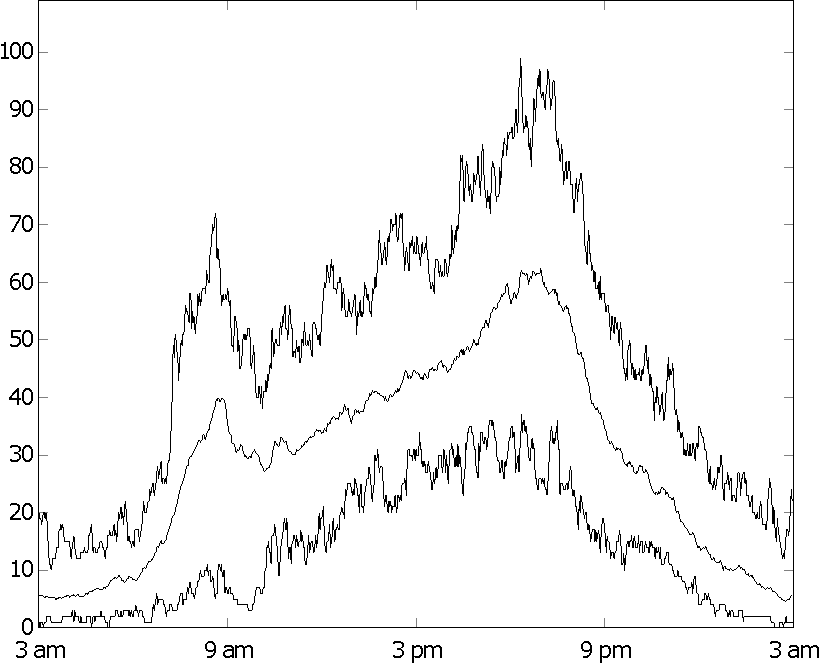
\includegraphics[width=0.8\textwidth]{graphic/Trip_Distribution}
	\caption{Distribution of trips (\cite[p.~62]{Kaiser}, \cite[p.~62]{Knoll})}
	\label{fig:trip_distribution}
\end{figure}

We aim to receive customers with several alternative routes. All routes of the same customer lie in a similar time window. Therefore we first create a set of customers. For each customer we determine a start and end position and a start time. The distribution of the customers' start times is similar to the distribution of the trips in \Cref{fig:trip_distribution}. We do not make the customers to be simple copies of the given trip set over a full instance. Instead we set the start and end positions randomly. We split the full instances into time periods of one hour, starting at each full hour. For each time period we create customers as follows:
\begin{enumerate}
	\item Determine the average number $k$ of trips starting in this time period by the given distribution.
	\item Take a sample of $k$ trips out of $\widehat{\mathcal{T}}$, use their start positions and times for the customers.
	\item Use the end positions of another sample of $k$ trips as end positions for the customers.
	\item Shift all start times by a full hour such that they start in the respective time period.
\end{enumerate}

With this procedure we create the customer set $\mathcal{C}$ with a preliminary start and end position and start time for each customer. Note that in general this preliminary start time does not coincide with $\zstart_c$ which is used in the mathematical models.

\paragraph{Route Creation} \parfill

For each customer we need a set of multimodal routes. Each route roughly starts at the preliminary start time of its customer. It further contains at least one car trip. For each customer there are routes with more than one car trip. In reality, such a route comprises a car trip, a public transport trip and then another car trip. Optionally, there are walking trips in-between. This is the only realistic possibility to gain routes with more than one car trip. Neither two car trips in a row nor a car trip between two public transport trips are a desirable option. The existence of routes with more than one car trip is crucial in order to test the developed solution approaches completely.

The multimodal routes are created with the open source software Open\-Trip\-Planner (cf.~\cite{OTP}). The input for this software is a start and end position and a start time. For each input, it provides several alternative multimodal routes, that comprise car, public transport and walking trips. A great restriction of these route is that they contain only one car trip and this car trip is always at the beginning. In order to receive the required test instances, we have to think of appending a car trip to the existing routes in a realistic way. For this, we do a reverse search from the end point to the start point and identify the station at which the public transport trip starts. Then we search for a multimodal route to this station and append a car trip from this station to the end position. This gives us a multimodal route that starts and ends with a car trip.

For each customer, we are given a start and end position and a start time. We create the routes as follows:
\begin{enumerate}
	\item Request a reverse search from the end position to the start position. Restrict the search to 3 alternative routes. For each alternative, identify the station where the first public transport trip starts.
	\item For each station, request a search from the start position to the station. Restrict the search to one alternative. Append a direct car trip from the station to the end position.
	\item Request a search from the start position to the end position. Restrict the search to 3 alternatives.
	\item Create a route with a direct car trip from the start to the end position.
\end{enumerate}

We use the customer start time as the start time for each search request. From each route, we extract the car trips. They are the only trips that are part of the problem input. With this procedure we create the multimodal route set~$\mathcal{M}$ and the trip set~$\mathcal{T}$ with up to 7 alternative routes and 10 trips for each customer.

\paragraph{Vehicles and Refuel Points} \parfill

Besides trips, a test instance contains vehicles and refuel points. Depending on the requested vehicle number, we take a sample of the previous vehicle set. If this does not suffice, \ie the requested vehicle number is greater than the vehicle set, we additionally create vehicles with the trips' end positions as starting positions of the vehicles. Since we do not have further information about the availability of the vehicles, we choose 2:00~am as the starting time of all vehicles. For the refuel point set, we use a sample of the existing refuel point set with the requested size.

\section{Fuel and Cost}
\label{sec:fuel_cost}

We need to determine the distances and times between two points for the fuel states and the costs. We compute these values with the open source software Open\-Source\-Routing\-Machine (cf.~\cite{OSRM}). The input are start and end positions and it provides the time and distance between each pair of start and end positions. We request the distances~$d$ and the times~$t$ for
\begin{align*}
	& d_{s,t} && t_{s,t} && \text{for all } s\in\mathcal{V}\cupdot\mathcal{T}\cupdot\mathcal{R}, t\in\mathcal{T}\cupdot\mathcal{R} \\
	& d_t && t_t && \text{for all } t\in\mathcal{T}
\end{align*}

and set the end times ${\zend_t := \zstart_t + t_t}$ for ${t\in\mathcal{T}}$.

\paragraph{Fuel States} \parfill

We assume that the fuel consumption depends linearly on the driven distance of the electrically powered vehicles and the refuel rate depends linearly on the time the vehicle stays at the refuel point. The fuel state of a vehicle is always in the interval $[0,1]$. We introduce the constants $v^{\operatorname{range}}$ which describes the maximal range of a vehicle and $v^{\operatorname{refuel}}$ which describes the maximal refueling time. Therefore the fuel consumption is given by
\begin{align*}
	\fd_{s,t} := \frac{d_{s,t}}{v^{\operatorname{range}}} && \text{for } s\in\mathcal{V}\cupdot\mathcal{R}\cupdot\mathcal{T}, t\in\mathcal{R}\cupdot\mathcal{T} && && \ft_t := \frac{d_t}{v^{\operatorname{range}}} && \text{for } t\in\mathcal{T}.
\end{align*}

The refuel rate is fiven by
\begin{align*}
	\ft_r := -\frac{\zstart_t - \zend_s - t_{s,r} - t_{r,t}}{v^{\operatorname{refuel}}} && \text{for all } r\in\Rst.
\end{align*}

Since we do not have further information about the fuel states of the vehicles, we set
\begin{align*}
	f^0_v := 1 && \text{for all } v\in\mathcal{V}.
\end{align*}

As realistic values we assume that the vehicle range is 135km and the refueling time is 8h. Therefore we set ${v^{\operatorname{range}} =}$~135,000 and ${v^{\operatorname{refuel}} =}$~28,800.

\paragraph{Costs} \parfill

The costs also depend linearly on the driven distance. The constant $c^{\operatorname{meter}}$ describes the cost for each meter a vehicle drives. Thus we set
\begin{align*}
	\cd_{s,t} := c^{\operatorname{meter}}\cdot d_{s,t} && \text{for } s\in\mathcal{V}\cupdot\mathcal{R}\cupdot\mathcal{T}, t\in\mathcal{R}\cupdot\mathcal{T} && && \ct_t := c^{\operatorname{meter}}\cdot d_t && \text{for } t\in\mathcal{T}.
\end{align*}

We set the constants ${c^{\operatorname{meter}} =}$~1 and ${\cv =}$~50,000.

The only cost left is the route cost. As mentioned in \Cref{sec:problem_description}, we use the route cost in order to model a realistic customer behavior. It contains the cost for public transport and the user inconvenience that arises if the customer chooses this route. We approximate the public transport cost in comparison to the cost for car sharing. The constant $c^{\operatorname{public}}$ describes the cost for using public transport. The main user inconveniences are the total travel time and the walking time. The constants $c^{\operatorname{time}}$ and $c^{\operatorname{walk}}$ describe the respective penalty costs.

Based on the charges of Car2Go (cf.~\cite{Car2Go}), we assume that a customer pays in average 0.50 euros per kilometer driving with a car. Due to the public transport provider in Stuttgart (cf.~\cite{VVS}), we assume that a customer pays in average 6 euros per hour using public transport. In order to compare the user inconveniences, we additionally charge 10 euros per hour for the total travel time and 10 euros per hour walking.

\newpage

\paragraph{Example} \parfill

In order to illustrate the procedure that we have developed before, we show an example of a multimodal route.

\begin{example}
\label{ex:example_route}

Consider that the route as described in \Cref{tab:exemplary_route} has been developed in \Cref{sec:trip_creation}. 

\begin{table}[htb]
	\centering
	\begin{tabular}{cccccc}
		\toprule
		Time & Mode & $d_t$ & $\ct$ & $\croute$ & Cost \\
		\midrule
		8:00 - 8:12 & Car & 6km & 6000 & & 3.00 euros \\
		8:12 - 8:15 & Walk & & & 1000 & 0.50 euros \\
		8:15 - 8:25	& Subway & & & 2000 & 1.00 euros \\
		8:25 - 8:28 & Wait & & & & \\
		8:28 - 8:33 & Bus & & & 1000 & 0.50 euros \\
		8:33 - 8:39 & Walk & & & 2000 & 1.00 euros \\
		8:39 - 8:45 & Car & 3km & 3000 & & 1.50 euros \\
		\bottomrule
	\end{tabular}
	\caption{Route according to \Cref{ex:example_route}}
	\label{tab:exemplary_route}
\end{table}

Only the car trips of this route are part of the input. Thus we have $t_1,t_2\in\mathcal{T}$. We call the route ${m=\left(t_1,t_2\right)}$ and the associated customer $c\in\mathcal{C}$. The trips have the values:
\begin{align*}
	\zstart_{t_1} = \text{8:00pm} && \zend_{t_1} = \text{8:12pm} && \ct_{t_1} = 6000 && \ft_{t_1} = 0.044 \\
	\zstart_{t_2} = \text{8:39pm} && \zend_{t_2} = \text{8:45pm} && \ct_{t_2} = 3000 && \ft_{t_2} = 0.022
\end{align*}

The total travel time amounts 0:45 hours. Thus, the route cost comprises a penalty of 15,000 for the total travel time, 3,000 for the walking time and 3,000 for the public transport cost. In summary we have ${\croute_m =}$~21,000.

\end{example}